The identification of rich wind resources have become important together with the increasing focus on green energy \cite{WindPowerGenerationUsingANN}. It can come as no surprise that the meteorological factors like wind speed and air density have an impact on the wind power. Figure~\ref{fig:energyGeneration} shows how the monthly wind power increases with the monthly average wind speed for their location --- we expect to see a similar relationship. 

\begin{figure}[h!]
\centering
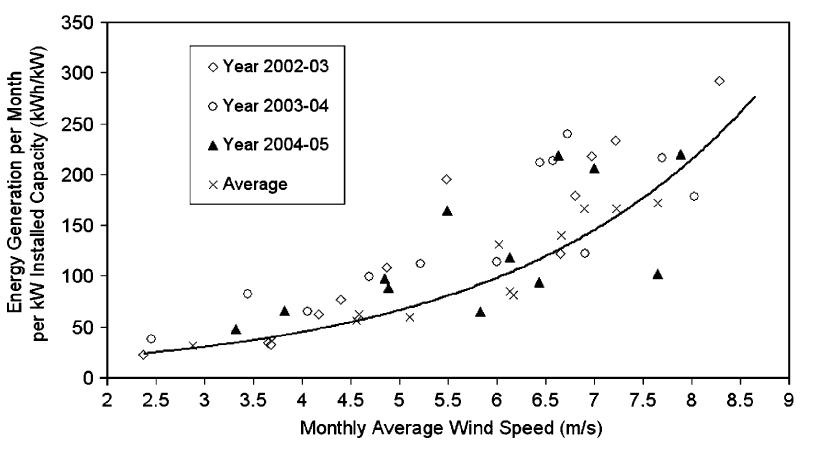
\includegraphics[width=0.8\linewidth,natwidth=898,natheight=587]{billeder/EnergyGenerationVsWindSpeed.png}
\caption{The influence of wind speed on the wind power \cite{WindPowerGenerationUsingANN}}
\label{fig:energyGeneration}
\end{figure} 

\subsubsection{Windmill Placement}
\label{sec:windmillPlacement}
It is important to analyse and predict the wind power at a certain location before placing actual windmills. Before making a substantial investment in a new wind farm it is of utmost importance to put it in the best possible location in relation to wind statistics, e.g. wind speed and how often the winds change in power and direction at the position. In \cite{4} they use a Measure-Correlate-Predict (MCP) method to predict wind statistics based on large amount of geographical-, weather- and historical data so that the farms can be placed best possible. These algorithms are heavy and will do calculations on sensor data directly from the location for months before giving any results. Time is not an issue because the company need to know for certain that the location will make the wind mills produce to the best or their ability.

Another approach is seen in \cite{WindPowerGenerationUsingANN} where wind speed, relative humidity and generation hours of the windmills are used as input for an Artificial Neural Network. Wind energy is proportional to air density where the more "heavy" air contributes to the windmill turbine receiving more energy, thus the wind power will vary together with the specific density and wind speed by the formula:

\begin{center}
$Power from Wind=\frac{1}{(2)}*\rho*A*V^3$
\end{center}

\noindent where $\rho = $ air density, A = area of the wind turbine and V = wind speed.
\newline
\noindent The wind speed is strengthened by the air density. Moist air is lighter than dry air because water molecules are less dense than the molecules in dry air such as oxygen and nitrogen. This basically means that the more air molecules like oxygen and nitrogen the more wind energy \cite{AirDensityInForecast}.
The air density depends on pressure and temperature but is also influenced by relative humidity. The parameters are necessary to investigate when attempting to forecast the wind power.

The last parameter in their prediction algorithm is generation hours that is the period in which the turbines produce power. The number of hours are influenced by for instance mechanical breakdowns, scheduled maintenance and low wind speeds. It is clear that the more generation hours the more energy is produced as seen in Figure~\ref{fig:energyGenerationFromHours}. The generation hours are hard to predict but can be calculated from past years uptime together with the expectations of the company delivering the windmills.  

\begin{figure}[h!]
\centering
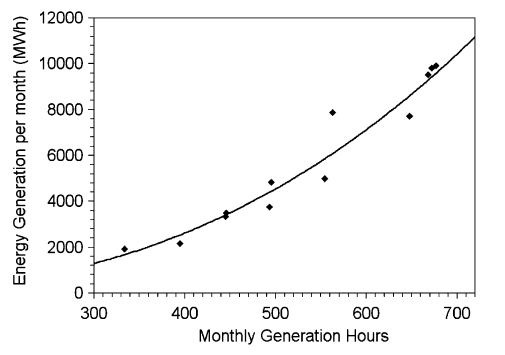
\includegraphics[width=0.8\linewidth,natwidth=898,natheight=587]{billeder/GenerationHourVSGeneration.png}
\caption{The influence of generation hours on energy production \cite{WindPowerGenerationUsingANN}}
\label{fig:energyGenerationFromHours}
\end{figure} 

The Artificial Neural Network trains on a 3-year dataset containing the mentioned input parameters. The input parameters are during the training compared to the output variable which is the wind power output of the turbine. See figure~\ref{fig:annArchitecture} for the architecture.
\\[0.5cm]
\begin{figure}[h!]
\centering
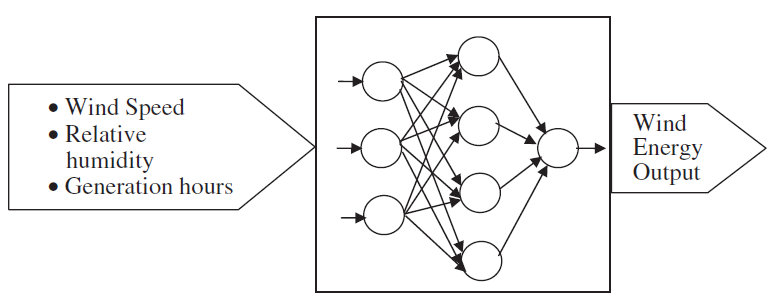
\includegraphics[width=0.7\linewidth,natwidth=898,natheight=587]{billeder/ANNwindSpeedPrediction.png}
\caption{Artificial Neural Network architecture from \cite{WindPowerGenerationUsingANN}}
\label{fig:annArchitecture}
\end{figure}

\subsubsection{Nearest Neighbour Approach}
Prediction can be done by using an algorithm that produces weighted nearest-neighbour tables to generate wind power curves based on available wind speed and direction from an online weather-data source. The weighted approach allows the algorithm to adapt to seasonal changes by weighting newest results highest, and the power curves makes it possible to use the algorithm on different wind farms. This prediction is used to schedule jobs in data centres which is described in Section~\ref{sec:greeEnergyProductionIntroduction}.

The time perspective and data of the algorithm is comparable to our specific purpose. The ANN dataset will consist of enough historical data fetched from online sources to make prediction possible.

\subsubsection{Summary}
It is described how the weather influences the wind power and what parameters are necessary to consider when doing the prediction. An Artificial Neural Network for prediction of wind power is presented and the concept of generation hours is discussed. The generation hours could help the network to forecast the wind power but since we are attempting to forecast the wind power for all of Western Denmark it seems unrealistic due to the many windmills in Denmark 

Furthermore, examples of how these predictions are used today is described. They are mainly used for placement planning of wind mill farms. Some knowledge can be transferred to our specific purpose but decision making in real-time cannot rely on heavy algorithms that will do calculations for days on data directly from the location. We must deliver accurate estimates without delaying the traders work.